\documentclass[conference]{IEEEtran}
% If the IEEEtran.cls has not been installed into the LaTeX system files, 
% manually specify the path to it:
% \documentclass[conference]{../sty/IEEEtran} 
\usepackage[brazil]{babel}
\usepackage{amsmath}
\usepackage{multirow}
\usepackage[utf8]{inputenc}
\usepackage[T1]{fontenc}
\usepackage{graphicx}
\usepackage{adjustbox}

% correct bad hyphenation here
\hyphenation{op-tical net-works semi-conduc-tor IEEEtran}

\begin{document}
	
	% paper title
	\title{Comparação de Modelos de Redes Neurais Artificiais sobre Problemas de Benchmark}
	
	
	% author names and affiliations
	% use a multiple column layout for up to three different
	% affiliations
	\author{\authorblockN{Victor São Paulo Ruela \\}
		\authorblockA{Programa de Pós-Graduação em Engenharia Elétrica\\
			Universidade Federal de Minas Gerais\\
			Belo Horizonte, Brasil\\
            Email: victorspruela@ufmg.br}}
	
	% avoiding spaces at the end of the author lines is not a problem with
	% conference papers because we don't use \thanks or \IEEEmembership
	
	% use only for invited papers
	%\specialpapernotice{(Invited Paper)}
	
	% make the title area
	\maketitle
	
	\begin{abstract}
		Este trabalho tem como objetivo avaliar o desempenho de diferentes modelos de redes neurais artificiais estudados durante a disciplina sobre bases de dados de benchmark presentes na literatura. Serão considerados o Perceptron, Adaline, Redes RBF, ELM e ELM com aprendizado Hebbiano. Para três problemas de regressão e classificação binária escolhidos, um experimento foi desenhado seguindo as recomendações da literatura. Os resultados de cada modelos são comparados por meio de testes estatíscticos para as metrícas AUC (classficação) e erro quadrático médio (regressão). Os resultados mostraram que, em geral, o ELM obteve um excelente desempenho para todas as bases de dados consideradas em relação aos demais modelos avaliados. Além disso, ficou evidente a dificuldade de se trabalhar com o RBF, o qual aparenta necessitar de bastante ajuste de seus hiper-parâmetros. Bons resultados também foram obtidos para o ELM Hebbiano, mostrando o potencial desta abordagem para problemas de classificação linearmente separáveis.
	\end{abstract}

	\section{Introdução}
	A Rede Neural Artificial (RNA) é uma classe de modelos muito popular em problemas de classificação, reconhecimento de padrões, regressão e predição~\cite{jain1996artificial}. Inspirado pelas características do cérebro humano, elas possuem como elementos básicos neurônios artificiais capazes de executar operações matemáticas, representando desta forma modelos de neurônios biológicos. Através de sua organização em diferentes estruturas de rede, tais modelos são capazes de se adaptar e representar funções matemáticas bastante complexas. 
	
	Neste trabalho será feita uma comparação entre diferentes modelos de RNAs: Perceptron, Adaline, Redes RBF, ELM e ELM com aprendizado Hebbiano. Para isso, um experimento será desenhado para comparar estatisticamente o seu desempenho sobre diferentes bases de dados de \textit{benchmark} disponíveis na literatura. Serão considerados tantos problemas de regressão e classificação, como forma de se explorar melhor a característica dos modelos considerados. 
	

	\section{Revisão da literatura}
	Nesta seção é feita uma breve descrição dos modelos de RNAs utilizados neste trabalho.
	
	\subsection{Perceptron}
	Proposto inicialmente por Rosenblatt~\cite{rosenblatt1957perceptron}, este é um modelo geralmente utilizado para a solução de problemas de classificação lineares. No seu trabalho original, o autor descreve formas de adaptação dos parâmetros, ou pesos, da rede com o objetivo de reduzir a discrepância entre as saídas esperadas e estimadas e aprender associações entre os neurônios, o que é a base da indução para diversos algoritmos atuais. Este trabalho é considerado um marco na literatura por diversos autores.
	
	Se considerarmos uma função de ativação contínua e diferenciável, os pesos da rede poderão ser inferidos de forma explícita, através do cálculo da pseudo-inversa, ou pelo algoritmo do gradiente descendente~\cite{hertz1991introduction}. Vale a pena ressaltar que a covergência destas abordagens está condicionada aos dados utilizados para treinamento serem linearmente independentes~\cite{hertz1991introduction}.
	
	\subsection{Adaline}
	O Adaline foi inicialmente desenvolvido por Widrow em 1960~\cite{widrow1960adaptive}, sendo principamente aplicado em problemas de regressão lineares. Assim como o Perceptron, originalmente este modelo considera somente um neurônio MCP em sua formulação, entretando sua função de ativação é a identidade. Seu treinamento é formulado como um problema de otimização com custo quadrático, onde originalmente foi utilizado o algoritmo do gradiente descendente para sua solução. 
	
	Para este agoritmo, em cada iteração é dado um passo na direção oposta ao gradiente da função objetivo, resultanto em uma convergência gradual para o mínimo do problema. Este gradiente pode ser calculado de forma análitica para a estrutura de rede do Adaline, o qual é no fim proporcional à diferença entre os valores estimados e reais~\cite{widrow1960adaptive}, bastante similar ao Perceptron simples. É fácil notar que o treinamento também pode ser realizado de forma direta através do cálculo da pseudo-inversa dos dados de entrada, já que este é um problema de mínimos quadrados~\cite{haykin2007neural}.
	
	\subsection{Redes RBF}
	As redes RBF foram inicialmente introduzidas por~\cite{broomhead1988multivariablefi} e são caracterizadas por um aprendizado que envolve duas etapas: (i) aplicar uma transformação aos padrões para um espaço onde a probabilidade de serem linearmente separáveis é alta (ii) encontrar os pesos usando o estimador mínimos quadrados usado no Perceptron simples. Essa estrutura pode ser representada por um rede de três camadas, onde sua camada escondida é reponsável pela transformação não-linear das entradas para o novo espaço, geralmente para uma dimensão muito alta. 
	
	Essa transformação é justificada pelo teorema de Cover sobre a separabilidade de padrões~\cite{cover1965geometrical}, o qual diz que um problema de classificação complexo projetado não-linearmente para um espaço de alta dimensão é mais provável de ser separável do que em um espaço de baixa dimensão, desde que o espaço não seja densamente povoado. Boa parte da teoria, que é relacionada ao campo de interpolação multivariável, considera um kernel baseado na função Gaussiana, que é uma classe importante de RBFs. Teoricamente, as redes RBF podem ser consideradas um aproximador universal de funções contínuas se a RBF é selecionada apropriadamente~\cite{poggio1990networks, park1991universal, liao2003relaxed}.
	
	\subsection{ELM}	
	Inicialmente proposto por~\cite{huang2004extreme}, as máquinas de aprendizado extremo (ELM) são redes neurais com uma única camada escondida, as quais possuem o atrativo de poucos parâmetros a serem ajustados, generalização maior ou similar e redução do tempo de treinamento das redes em relação aos métodos convencionais. Seu treinamento é baseado na teoria de minimização de risco empírico, necessitando de somente uma iteração para este processo, evitando múltiplas iterações e algoritmos de otimização local~\cite{ding2015extreme}. 
	
	ELMs são capazes de definir adaptivamente o número neurônios da rede e aleatoriamente escolher os pesos das entradas e viéses da camada escondida~\cite{huang2006extreme}. Isso faz com o que a rede possa ser considerada como um sistema linear, o qual pode ser calculado de forma analítica através de uma operação de inversão da matriz de pesos da camada de saídas~\cite{huang2006extreme}. Essa característica permite uma drástica redução do esforço computacional do treinamento, geralmente de 10 vezes ou mais~\cite{deng2010research}. 
	
	\section{Metodologia}
	\subsection{Bases de Dados}
	Neste trabalho serão consideradas três bases de dados referentes a problemas de classificação binários e regressão multivariada disponíveis no repositório da UCI \cite{dua2019}, totalizando seis problemas. Antes do treinamento, os dados de entrada serão normalizados para o intervalo $[0,1]$ e filtrados para remoção de valores inválidos. Um sumário das bases de dados consideradas pode ser vista na Tabela \ref{tab:datasets}.
	
	\begin{table}[thpbh]
		\caption{Principais características das bases de dados utilizadas}
		\label{tab:datasets}
		\centering
		\begin{tabular}{l|c|c|c|}
			\cline{2-4}
			& \textbf{Instâncias} & \textbf{Atributos} & \textbf{Proporção} \\ \hline
			\multicolumn{1}{|l|}{\textbf{Breast Cancer}}   & 569                 & 32                 & 0.66                           \\ \hline
			\multicolumn{1}{|l|}{\textbf{Liver Disorder}}  & 245                 & 6                  & 0.58                           \\ \hline
			\multicolumn{1}{|l|}{\textbf{Statlog (Heart)}} & 270                 & 13                 & 0.66                           \\ \hline
			\multicolumn{1}{|l|}{\textbf{Boston Housing}}  & 506                 & 13                 & N/A                            \\ \hline
			\multicolumn{1}{|l|}{\textbf{Wine Quality (Red)}}      & 1599                 & 11                 & N/A                            \\ \hline
			\multicolumn{1}{|l|}{\textbf{Diabetes}}        & 442                 & 10                 & N/A                            \\ \hline
		\end{tabular}
	\end{table}
	
	\subsection{Desenho do experimento}
	A partir das recomendações para desenho de experimento para comparação de algoritmos proposta em \cite{salzberg1997comparing}, a seguinte metodologia será adotada:
	\begin{itemize}
		\item Para cada base de dados:
			\begin{enumerate}
			\item Particionar os dados $D$ em $k$ partições para validação cruzada, mantendo a mesma proporção entre os rótulos
			\begin{enumerate}
				\item Criar o conjunto de treino $T = D - k$
				\item Para cada modelo:
				\begin{enumerate}
					\item Executar busca exaustiva com validação cruzada de $z$ sobre $T$ para os coeficientes de regularização $\lambda$ \label{item:grid-search}
					\item Escolher $\lambda$ que obtém o melhor ajuste médio 
					\item Avaliar a métrica do modelo sobre $k$
				\end{enumerate}
			\end{enumerate}
			\item Estimar o intervalo de confiança de 95\% do valor médio da métrica sobre $k$ usando \textit{bootstraping}
		\end{enumerate}
	\end{itemize}
	
	O número de partições consideradas será de $k=10$. Para o item \ref{item:grid-search}, serão considerados um número fixo de valores igualmente espaçados dentro de um intervalo pré-definido. Além disso, serão considerados $z=5$ partições, como forma de controlar um pouco o tamanho do experimento. Serão consideradas as métricas AUC para classificação e erro quadrático médio (MSE) para regressão, respectivamente. A implementação deste experimento, bem como dos modelos utilizados, será feita em Python e utilizando principalmente os pacotes \textit{numpy} \cite{harris2020array} e \textit{scikit-learn} \cite{scikit-learn}. 
	
	Os algoritmos ELM e RBF foram implementados seguindo as notas de aula do professor, sendo que o RBF irá considerar o \textit{k-means} para o cálculo dos centros e raios. O Percepton utilizado está disponível na biblioteca \textit{scikit-learn} diretamente, suportando o uso de regularização. Já o Adaline foi implementado usando o algoritmo MLP disponível no \textit{scikit-learn}, considerando um único neurônio na camada escondida e aprendizado via o algoritmo do gradiente estocástico. Isso foi necessário uma vez que esta implementação suporta o uso de regularização. O experimento será realizado em um Notebook Intel Core i7 Quad Core com 8Gb de memória RAM, sendo que o uso de paralelização será utilizado sempre que possível visto a enorme quantidade de vezes que os modelos serão treinados.
	
	\subsection{ELM Hebbiano}
	Uma variação presente na literatura para controlar a generalização do ELM consiste no uso do aprendizado Hebbiano após a camada escondida \cite{horta2015aplicaccao}. Conforme sugerido pelo autor, podemos substituir o cálculo da pseudo-inversa da matriz de projeção aleatória por um Perceptron Hebbiano com pesos normalizados. Será considerada o algoritmo de aprendizado Hebbiano considerando somente um neurônio, similiar ao Perceptron simples. Essa abordagem é melhor descrita em \cite{fernandez2011direct}, da qual podemos retirar a seguinte regra para problemas de classificação binários:
	\begin{equation}
		w = \frac{ \sum^{N}_{i=1} y_i\textbf{h}_i}{\left\|  \sum^{N}_{i=1} y_i\textbf{h}_i \right\| }
	\end{equation}
	onde $\textbf{h}_i$ é á $i$-ésima linha da matriz de projeção aleatória do algoritmo ELM original. É importante ressaltar que esta regra assume que os dados foram normalizados para possuir média zero e desvio padrão unitário. Para validar a implementação, o algoritmo foi executado sobre duas bases de dados simples e 100 neurônios na camada escondida, cujos resultados podem ser vistos na Figura \ref{fig:box-hebb-test}.
	
	\begin{figure}[thpbh]
		\centering
		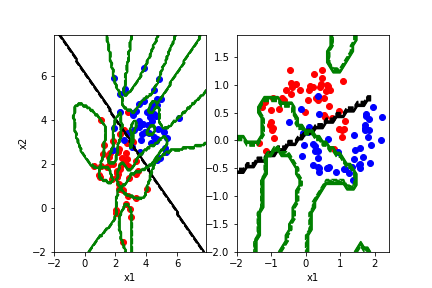
\includegraphics[width=0.5\textwidth]{figures/hebb_test.png}
		\caption{Comparação entre o ELM original (verde) e sua versão com aprendizado Hebbiano (preto) em um problema linearmente e outro não-linearmente separável}
		\label{fig:box-hebb-test}
	\end{figure}
	
	Através destes resultados, podemos concluir que o uso do aprendizado Hebbiano é capaz de atingir a regularização desejada. Entretanto, nota-se que a superfície de separação torna-se predominantemente linear, de forma que seja esperado que esta abordagem possua desempenho limitado para problemas que não sejam linearmente separáveis.
	
	
	\section{Resultados}
	
	\subsection{Problemas de Classificação}
	Para os problemas de classificação foram considerados os algoritmos Perceptron, RBF, ELM e ELM com apredizado Hebbiano. Foi estabelecido um número fixo de 20 neurônios na camada escondida e não foi aplicada regularização ao ELM Hebbiano. 50 valores para o coeficiente de regularização foram escolhidos no intervalo $[0,1]$. Os gráficos boxplot para cada conjunto de dados considerado é exibido nas Figuras \ref{fig:box-Breast Cancer}, \ref{fig:box-Liver-Disorder} e \ref{fig:box-statlog-heart}. Os intervalos de confiança calculados são exibidos na Tabela \ref{tab:classification}.
	
	\begin{figure}[thpbh]
		\centering
		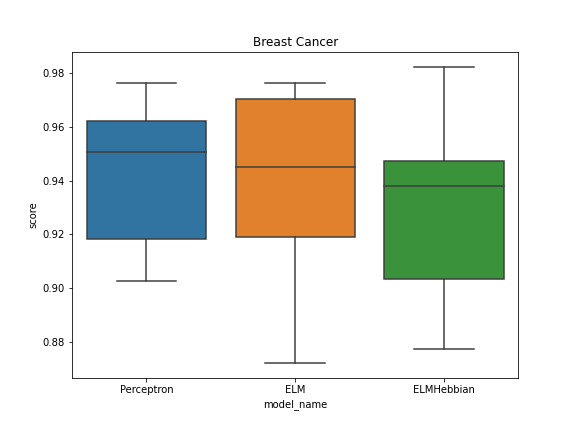
\includegraphics[width=0.5\textwidth]{figures/Breast Cancer_scores.png}
		\caption{Boxplots para a base de dados \textit{Breast Cancer}. Intervalos de confiança de 95\% para a média são exibidos em preto.}
		\label{fig:box-Breast Cancer}
	\end{figure}
	
		\begin{figure}[thpbh]
		\centering
		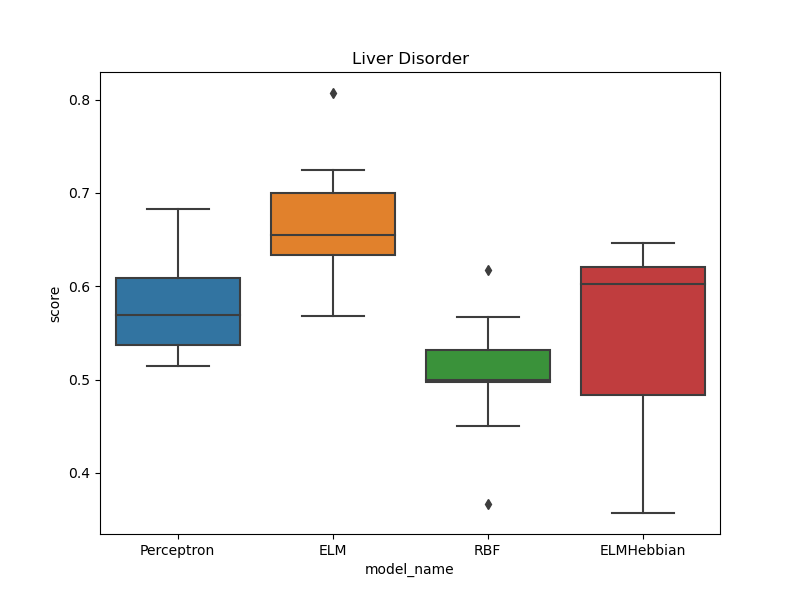
\includegraphics[width=0.5\textwidth]{figures/Liver Disorder_scores.png}
		\caption{Boxplots para a base de dados \textit{Liver Disorder}. Intervalos de confiança de 95\% para a média são exibidos em preto.}
		\label{fig:box-Liver-Disorder}
	\end{figure}	
	
	
	\begin{figure}[thpbh]
		\centering
		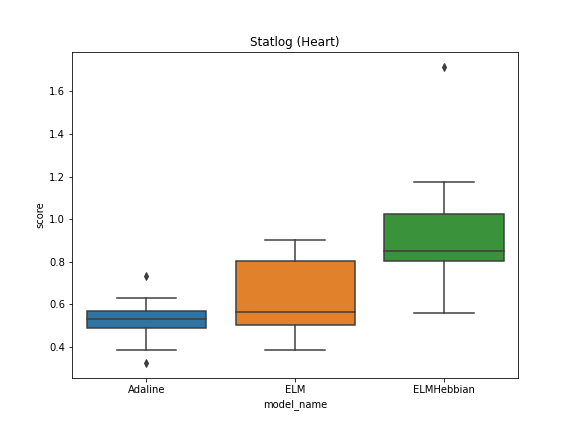
\includegraphics[width=0.5\textwidth]{figures/Statlog (Heart)_scores.png}
		\caption{Boxplots para a base de dados \textit{Statlog (Heart)}. Intervalos de confiança de 95\% para a média são exibidos em preto.}
		\label{fig:box-statlog-heart}
	\end{figure}
	
	A partir destes resultados, podemos chegar às seguintes conclusões:
	\begin{itemize}
		\item Para um intervalo de confiança de 95\%, podemos afirmar que todos os algoritmos possuem desempenho médio superior ao modelo RBF nas bases de dados avaliadas.
		\item Para a base de dados \textit{Breast Cancer}, os modelos ELM e Perceptron obtiveram desempenhos bastante similares. Além disso, podemos afirmar que eles obtiveram desempenho médio superior ao ELM Hebbiano para o intervalo de confiança de 95\%.
		\item Para a base de dados \textit{Statlog (Heart)} não podemos rejeitar a hipótese de que os modelos ELM, ELM Hebbiano e Perceptron possuam desempenhos iguais para o intervalo de confiança de 95\%.
		\item Para a base de dados \textit{Liver Disorder}, podemos afirmar que para um intervalo de confiança de 95\%, o ELM possui desempenho superior aos demais modelos.
		\item Uma hipótese para o desempenho muito abaixo do esperado do RBF pode estar no número de neurônions escolhidos para a camada escondida. Este hiperparâmetro não foi ajustado para que a comparação com o ELM seja justa e também para limitar o tamanho do experimento a ser executado. 
		\item A diferença de desempenho entre o ELM e sua versão com aprendizado Hebbiano está no fato deste última poder estar resultando em uma regularização excessiva. Isso sugere que uma implementação diferente do modelo Hebbiano é indicado para controlar melhor a sua generalização.
		\item É interessante notar que para problemas lineares não houve uma perda muito grande na AUC média dos modelos ELM e ELM Hebbiano. Entretanto, nota-se uma maior variabilidade para este último modelo, o que sugere uma maior sensibilidade à base de dados em estudo. 
	\end{itemize}

	\begin{table*}[thpbh]
		\caption{Intervalos de confiança de 95\% calculados para a AUC média}
		\label{tab:classification}
		\centering
		\begin{tabular}{r|r|r|r|r|}
			\cline{2-5}
			\multicolumn{1}{l|}{}                          & \multicolumn{1}{c|}{\textbf{ELM}} & \multicolumn{1}{c|}{\textbf{ELM Hebbiano}} & \multicolumn{1}{c|}{\textbf{Perceptron}} & \multicolumn{1}{c|}{\textbf{RBF}} \\ \hline
			\multicolumn{1}{|r|}{\textbf{Breast Cancer}}   & \textbf{0.948 (0.935,0.963)}         & 0.887 (0.853,0.920)                           & \textbf{0.950 (0.930,0.971)}                & 0.512 (0.505,0.519)                  \\ \hline
			\multicolumn{1}{|r|}{\textbf{Liver Disorder}}  & \textbf{0.677 (0.621,0.733)}         & 0.582 (0.536,0.628)                           & 0.532 (0.509,0.553)                         & 0.515 (0.498,0.537)                  \\ \hline
			\multicolumn{1}{|r|}{\textbf{Statlog (Heart)}} & \textbf{0.812 (0.769,0.851)}         & 0.762 (0.698,0.819)                           & 0.772 (0.700,0.846)                         & 0.547 (0.522,0.569)                  \\ \hline
		\end{tabular}
	\end{table*}

	\subsection{Problemas de Regressão}
	Para os problemas de classificação foram considerados os algoritmos Adaline, RBF e ELM. Não foi possível realizar uma implementação do ELM Hebbiano que funcionasse com problemas de regressão, logo este modelo teve que ser descartado. Foi estabelecido um número fixo de 20 neurônios na camada escondida e a regularização foi considerada somente para todos os algoritmos. 50 valores de coeficiente de regularização foram escolhidos no intervalo $[0,1]$. Nenhum outro ajuste de hiper-parâmetro foi feito para o Adaline, sendo usados os valores padrão da biblioteca \textit{scikit-learn}. Os gráficos boxplot para cada conjunto de dados considerado é exibido nas Figuras \ref{fig:box-Boston-Housing}, \ref{fig:box-Wine} e \ref{fig:box-Diabetes}.  Os intervalos de confiança calculados são exibidos na Tabela \ref{tab:classification}.

	\begin{figure}[thpbh]
		\centering
		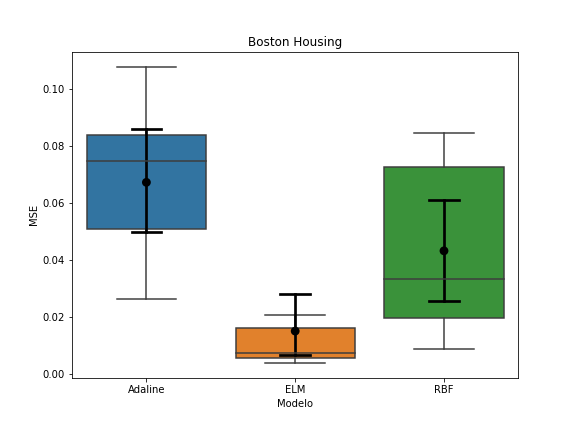
\includegraphics[width=0.5\textwidth]{figures/Boston Housing_scores.png}
		\caption{Boxplots para a base de dados \textit{Boston Housing}. Intervalos de confiança de 95\% para a média são exibidos em preto.}
		\label{fig:box-Boston-Housing}
	\end{figure}
	
	\begin{figure}[thpbh]
		\centering
		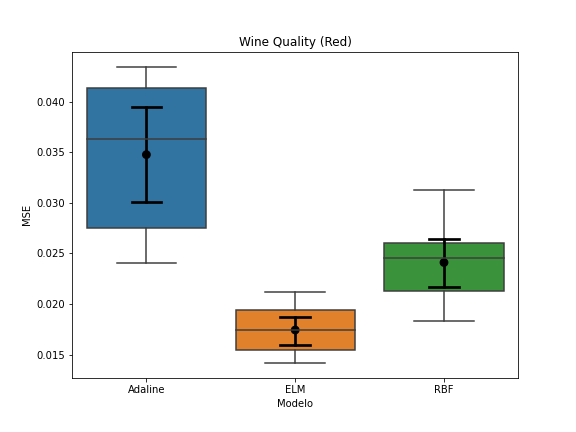
\includegraphics[width=0.5\textwidth]{figures/Wine Quality (Red)_scores.png}
		\caption{Boxplots para a base de dados \textit{Wine Quality (Red)}. Intervalos de confiança de 95\% para a média são exibidos em preto.}
		\label{fig:box-Wine}
	\end{figure}
	
	\begin{figure}[thpbh]
		\centering
		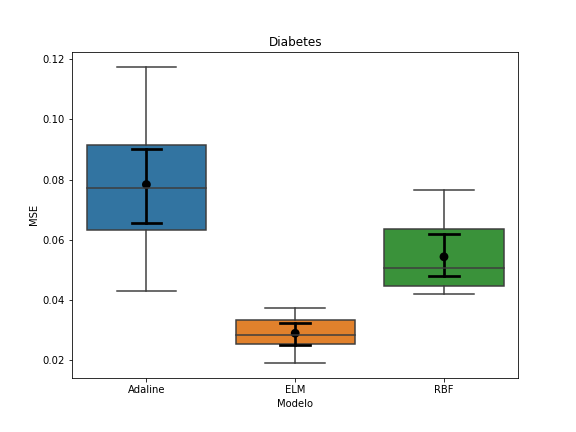
\includegraphics[width=0.5\textwidth]{figures/Diabetes_scores.png}
		\caption{Boxplots para a base de dados \textit{Diabetes}. Intervalos de confiança de 95\% para a média são exibidos em preto.}
		\label{fig:box-Diabetes}
	\end{figure}

	
	\begin{table*}[thpbh]
		\caption{Intervalos de confiança de 95\% calculados para o MSE médio}
		\label{tab:regression}
		\centering
%		\begin{adjustbox}{width=1\linewidth}
			\begin{tabular}{l|c|c|c|}
				\cline{2-4}
				& \textbf{Adaline} & \textbf{ELM}              & \textbf{RBF}     \\ \hline
				\multicolumn{1}{|l|}{\textbf{Boston Housing}} & 0.069 (0.039,0.096) & \textbf{0.012 (0.008,0.016)} & 0.044 (0.025,0.061) \\ \hline
				\multicolumn{1}{|l|}{\textbf{Diabetes}}       & 0.078 (0.066,0.091) & \textbf{0.029 (0.025,0.033)} & 0.054 (0.048,0.061) \\ \hline
				\multicolumn{1}{|l|}{\textbf{Wine Quality (Red)}}     & 0.037 (0.031,0.043) & \textbf{0.017 (0.016,0.019)} & 0.024 (0.022,0.026) \\ \hline
			\end{tabular}
%		\end{adjustbox}
	\end{table*}

	A partir destes resultados, podemos chegar às seguintes conclusões:
	\begin{itemize}
		\item Para um intervalo de confiança de 95\%, podemos afirmar que o ELM teve desempenho médio superior aos demais algoritmos para as bases de dados \textit{Diabeters} e \textit{Wine Quality (Red)}. Embora não podemos afirmar estatisticamente que o ELM seja superior, é importante notar que ele apresentou uma variabilidade muito menor.
		\item O Problema \textit{Boston Housing} é conhecido pela sua característica linear, o que explica os bons resultados obtidos para o Adaline.
		\item Ao contrário do que ocorrou para os problemas de classificação, o RBF obteve bons resultados quando utilizado para regressão.
		\item O Adaline possuiu um desempenho bem abaixo do esperado, apresentando muita variação e uma MSE médio superior se o problema apresentar comportamento predominantemente não-linear. Isso está de acordo com a característica deste modelo.
	\end{itemize}
	
	
	
	\section{Conclusões}
	
	Neste trabalho foi feita uma avaliação do desempenho dos modelos ELM, RBF, Adaline, Perceptron e ELM Hebbiano sobre bases de dados de benchmark presentes na literatura. A partir de um experimento desenhado para tal finalidade, os resultados foram comparados estatísticamente utilizando a técnica de \textit{bootstrapping} para a média das métricas AUC e erro quadrático médio, considerando um intervalo de confiança de 95\%. Destaca-se o excelente desempenho do ELM em todos os conjuntos de dados, tanto de regressão e classificação. É importante destacar também o desempenho muito abaixo do esperado para o RBF nos problemas de classificação, sugerindo a necessidade de um melhor ajuste do número de neurônios na camada escondida, por exemplo. Notou-se também que os modelos lineares avaliados obtiveram bons resultados dependendo da base de dados em questão, conseguindo atingir um desempenho estatisticamente equivalente aos demais.
	
	Uma surpresa foi o ELM Hebbiano, onde embora tenha sido usada uma abordagem bem simples de aprendizado Hebbiano, não apresentou um resultado muito inferior em relação ao ELM original para classificação. Destaca-se o fato de que não foi possível utilizar a estratégia de aprendizado Hebbiano com sucesso em problemas de regressão. Isso sugere que uma abordagem diferente deve ser utilizada nesta situação. Durante a execução do experimento, pôde ser observado também que o modelo RBF possui um tempo de treinamento muito maior que os demais. Isso fez com que ele fosse o gargalo de todo o experimento neste quesito, o que limitou um pouco o potencial de executar um número maior de partições para a validação cruzada, bem como avaliar um intervalo maior para o fator de regularização. 
	
	Como trabalhos futuros, é sugerido um ajuste fino de demais hiper-parâmetros do RBF como forma de tentar melhorar o seu desempenho. Além disso, também é interessante avaliar outras formas de aprendizado Hebbiano que poderiam ser utilizados com o ELM, bem como para melhorar seu poder de generalização e também ser aplicável a problemas de regressão com sucesso. Outra tarefa importante seria a realização de uma etapa de pré-processamento mais completa sobre bases de dados considerados, o qual não foi feita por restrições de tempo mas teria potencial para melhorar os resultados obtidos de todos os modelos.
		


    \bibliographystyle{unsrt}
	\bibliography{artigo2}
	
\end{document} 